\documentclass[a4paper, 11pt]{article} % Font size (can be 10pt, 11pt or 12pt) and paper size (remove a4paper for US letter paper)

\usepackage[protrusion=true,expansion=true]{microtype} % Better typography
\usepackage[a4paper, margin=3.5cm]{geometry} %Annina style
\usepackage{graphicx} % Required for including pictures
\usepackage{wrapfig} % Allows in-line images
\usepackage{enumitem} %%Enables control over enumerate and itemize environments
\usepackage{setspace}
\usepackage{amssymb, amsmath, mathrsfs,amsthm} %%Math packages
\usepackage{stmaryrd}
\usepackage{mathtools}
\usepackage{mathpazo} % Use the Palatino font
\usepackage[T1]{fontenc} % Required for accented characters
\usepackage{array}
\usepackage{bibentry}
\usepackage[round]{natbib} %%Or change 'round' to 'square' for square backers
% \usepackage{tikz}
\usepackage{comment}

\usepackage{lipsum}
\newenvironment{Answer}[1][Answer]
  {\proof[#1]\leftskip=1cm\rightskip=1cm}
  {\endproof}
  % \def\firstcircle{(140:-1.5cm) circle (1.5cm)}
  % \def\secondcircle{(210:1.75cm) circle (2.5cm)}
  % \def\thirdcircle{(330:1.75cm) circle (2.5cm)}


\setcitestyle{aysep={}}

\linespread{1.05} % Change line spacing here, Palatino benefits from a slight increase by default

\renewcommand{\qed}[0]{$\hfill\Box$} %%Box at end of proofs
\newcommand{\s}[0]{\mathcal{S}} %%Box at end of proofs
\renewcommand{\L}[0]{\mathcal{L}} %%Box at end of proofs
\newcommand{\V}[0]{\mathcal{V}} %%Box at end of proofs
\renewcommand{\t}[0]{\mathcal{A}} %%Box at end of proofs
\newcommand{\corner}[1]{\ulcorner#1\urcorner} %%Corner quotes
\newcommand{\tuple}[1]{\langle#1\rangle} %%Angle brackets
\newcommand{\set}[1]{\lbrace#1\rbrace} %%Set brackets
\newcommand{\interpret}[1]{\llbracket#1\rrbracket} %%Double brackets
%\DeclarePairedDelimiter\ceil{\lceil}{\rceil}    
\newcommand{\qpar}[0]{\par\hspace*{.2in}}


\newtheorem{innercustomthm}{}
\newenvironment{customthm}[1]
  {\renewcommand\theinnercustomthm{#1}\innercustomthm}
  {\endinnercustomthm}


\newtheoremstyle{theorem}
{}                % Space above
{}                % Space below
{\normalfont}        % Theorem body font % (default is "\upshape")
{}                % Indent amount
{\bfseries}       % Theorem head font % (default is \mdseries)
{}               % Punctuation after theorem head % default: no punctuation
{.18in}               % Space after theorem head
{}                % Theorem head spec
\theoremstyle{theorem}
\newtheorem{theorem}{}% theorem counter resets every \subsection
\renewcommand{\thetheorem}{T\arabic{theorem}}% Remove subsection from theorem counter representation


\newtheoremstyle{Pthm}
{}                % Space above
{}                % Space below
{\normalfont}        % Theorem body font % (default is "\upshape")
{.25in}                % Indent amount
{\bfseries}       % Theorem head font % (default is \mdseries)
{}               % Punctuation after theorem head % default: no punctuation
{.18in}               % Space after theorem head
{}                % Theorem head spec
\theoremstyle{Pthm}
\newtheorem{Pthm}{}% theorem counter resets every \subsection
\renewcommand{\thePthm}{P\arabic{Pthm}}% Remove subsection from theorem counter representation


\usepackage{calc}
\makeatletter
\newcommand{\labelalign@original@item}{}
\let\labelalign@original@item\item
\newcommand*{\labelalign@envir}{labelalign}
\newlength{\labelalign@totalleftmargin}
\newlength{\labelalign@linewidth}
\newcommand{\labelalign@makelabel}[1]{\llap{#1}}%
\newcommand{\labelalign@item}[1][]{%
  \setlength{\@totalleftmargin}%
       {\labelalign@totalleftmargin+\widthof{\textbf{#1 }}+.25in-\leftmargin}%
  \setlength{\linewidth}
       {\labelalign@linewidth-\widthof{\textbf{#1 }}-.25in+\leftmargin}%
  \par\parshape \@ne \@totalleftmargin \linewidth
  \labelalign@original@item[\textbf{#1}]%
}
\newenvironment{labelalign}
  {\list{}{\setlength{\labelwidth}{0in}%
           \let\makelabel\labelalign@makelabel}%
   \setlength{\labelalign@totalleftmargin}{\@totalleftmargin}%
   \setlength{\labelalign@linewidth}{\linewidth}%
   \renewcommand{\item}{\ifx\@currenvir\labelalign@envir
                           \expandafter\labelalign@item
                        \else
                           \expandafter\labelalign@original@item
                        \fi}}
  {\endlist}
\makeatother


\makeatletter
\renewcommand\@biblabel[1]{\textbf{#1.}} % Change the square brackets for each bibliography item from '[1]' to '1.'
\renewcommand{\@listI}{\itemsep=0pt} % Reduce the space between items in the itemize and enumerate environments and the bibliography

\lineskiplimit=-100pt\relax

\renewcommand{\maketitle}{ % Customize the title - do not edit title and author name here, see the TITLE block below
\begin{flushright} % Right align
{\LARGE\@title} % Increase the font size of the title

\vspace{10pt} % Some vertical space between the title and author name

{\@author} % Author name
\\\@date % Date

\vspace{30pt} % Some vertical space between the author block and abstract
\end{flushright}
}

%----------------------------------------------------------------------------------------
%	TITLE
%----------------------------------------------------------------------------------------

\title{\textbf{Revisions: TT2020}} % Subtitle

\author{\textsc{Introduction to Logic}\\ \em Benjamin Brast-McKie} % Institution

\date{\today} % Date

%----------------------------------------------------------------------------------------

\begin{document}

\maketitle % Print the title section

\thispagestyle{empty}

%----------------------------------------------------------------------------------------


% \vspace{.1in}
% \begin{customthm}{(NUMBER)}
%   CLAIM
% \end{customthm}

% \begin{Answer}
%   ANSWER
% \end{Answer}


\section*{HT2016: Problem 4}

\begin{center}
  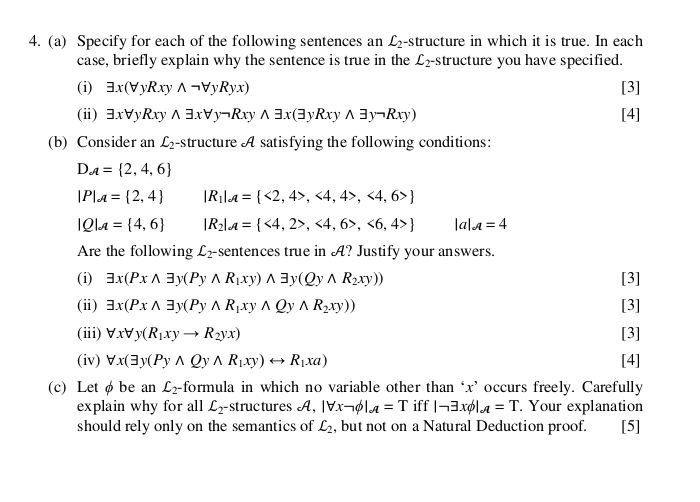
\includegraphics[width=1\textwidth]{Q4.png}
\end{center}

\section*{Solutions}

\vspace{.1in}
\begin{customthm}{(4.a.i)}
  $ \exists x
      ( \forall y Rxy \wedge \neg \forall y Ryx )$
\end{customthm}

\begin{Answer}
  % Let $ D = \set{0,1} $,
  %   and $ |R| = \set{ \tuple{0,0}, \tuple{0,1} } $.
\end{Answer}




\vspace{.1in}
\begin{customthm}{(4.a.ii)}
  $ \exists x
      \forall y Rxy \wedge
        \exists x
          \forall y \neg Rxy \wedge
      \exists x ( \exists y Rxy
        \wedge \exists y\neg Rxy )$
\end{customthm}

\begin{Answer}
  % Let $ D = \set{} $,
  %   and $ |R| = \set{} $.
\end{Answer}



 
\vspace{.1in}
\begin{customthm}{(4.b.i)}
  $ \exists x ( Px \wedge
      \exists y ( Py \wedge R_1xy ) \wedge
        \exists y (Qy \wedge R_2xy)) $
\end{customthm}

\begin{Answer}
  % True: 
  %   set $ |x|_\alpha = 4 $,
  %   $ |y|_\beta = 4 $ where $\beta$ differs from $\alpha$ at most in $y$,
  %   and $ |y|_\gamma = 6 $ where $\gamma$ differs from $\alpha$ at most in $y$.
\end{Answer}




\vspace{.1in}
\begin{customthm}{(4.b.ii)}
  $ \exists x ( Px \wedge
      \exists y ( Py \wedge R_1xy \wedge Qy \wedge R_2xy)) $
\end{customthm}

\begin{Answer}
  There are two cases to check since $x$ must be assigned to something in $ |P|_A = \set{2,4}$:
    
    \textit{Case 1:}
      set $ |x|_\alpha = 2 $.
      Again there are two cases to check since $y$ must be assigned to something in $ |P|_A $:

        \textit{Case 1.1:}
        set $ |y|_\beta = 2 $ where $\beta$ differs from $\alpha$ at most in $y$.
        Since $ \tuple{2,2} \notin |R_1|_A $, we know that
          $ |R_1xy|_A = F $, and so by the semantics for conjunction
          $ | Py \wedge R_1xy \wedge Qy \wedge R_2xy |_A = F $.

        \textit{Case 1.2:}
        set $ |y|_\beta = 4 $ where $\beta$ differs from $\alpha$ at most in $y$.
        Since $ \tuple{2,4} \notin |R_2|_A $, we know that
          $ |R_2xy|_A = F $, and so by the semantics for conjunction
          $ | Py \wedge R_1xy \wedge Qy \wedge R_2xy |_A = F $.

      Thus $|\exists y (Py \wedge R_1xy \wedge Qy \wedge R_2xy)|_A = F $ in either case,
        and so by the semantics for conjunction $|Px \wedge \exists y (Py \wedge R_1xy \wedge Qy \wedge R_2xy)|_A = F $.

    \textit{Case 2:}
      set $ |x|_\alpha = 4 $.
      Again there are two cases to check since $y$ must be assigned to something in $ |P|_A $:

        \textit{Case 2.1:}
        set $ |y|_\beta = 2 $ where $\beta$ differs from $\alpha$ at most in $y$.
        Since $ \tuple{4,2} \notin |R_1|_A $, we know that
          $ |R_1xy|_A = F $, and so by the semantics for conjunction
          $ | Py \wedge R_1xy \wedge Qy \wedge R_2xy |_A = F $.

        \textit{Case 2.2:}
        set $ |y|_\beta = 4 $ where $\beta$ differs from $\alpha$ at most in $y$.
        Since $ \tuple{4,4} \notin |R_2|_A $, we know that
          $ |R_2xy|_A = F $, and so by the semantics for conjunction
          $ | Py \wedge R_1xy \wedge Qy \wedge R_2xy |_A = F $.
      
      Thus $|\exists y (Py \wedge R_1xy \wedge Qy \wedge R_2xy)|_A = F $ in either case,
        and so by the semantics for conjunction $|Px \wedge \exists y (Py \wedge R_1xy \wedge Qy \wedge R_2xy)|_A = F $.

    Thus $|Px \wedge \exists y (Py \wedge R_1xy \wedge Qy \wedge R_2xy)|_A = F $ in either case, and so \textbf{(4.b.ii)} is false by the semantics for conjunction.

\end{Answer}




\vspace{.1in}
\begin{customthm}{(4.b.iii)}
  $\forall x
    \forall y ( R_1xy \rightarrow R_2yx )$
\end{customthm}

\begin{Answer}
  False:
\end{Answer}





\vspace{.1in}
\begin{customthm}{(4.b.iv)}
  $\forall x ( 
      \exists y ( 
        Py \wedge Qy \wedge R_1xy)
      \leftrightarrow R_1xa)$
\end{customthm}

\begin{Answer}
  True:
\end{Answer}



\vspace{.1in}
\begin{customthm}{(4.c)}
  Show that $|\forall x \neg \varphi|_A = |\neg\exists x \varphi |_A$.
\end{customthm}

\begin{Answer}[Proof]
  Letting $A$ be arbitrary, we may observe the following:
  \vspace{-1.25in}
  \begin{flalign*}
    |\forall x \neg \varphi|_A =1 & ~~\textit{iff}~~ |\neg \varphi|_A^\alpha = 1 ~\text{for all}~ \alpha
    \\    & ~~\textit{iff}~~ |\varphi|_A^\alpha = 0 ~\text{for all}~ \alpha
  \end{flalign*}

\end{Answer}





\section*{HT2019: Problem 6}

\begin{center}
  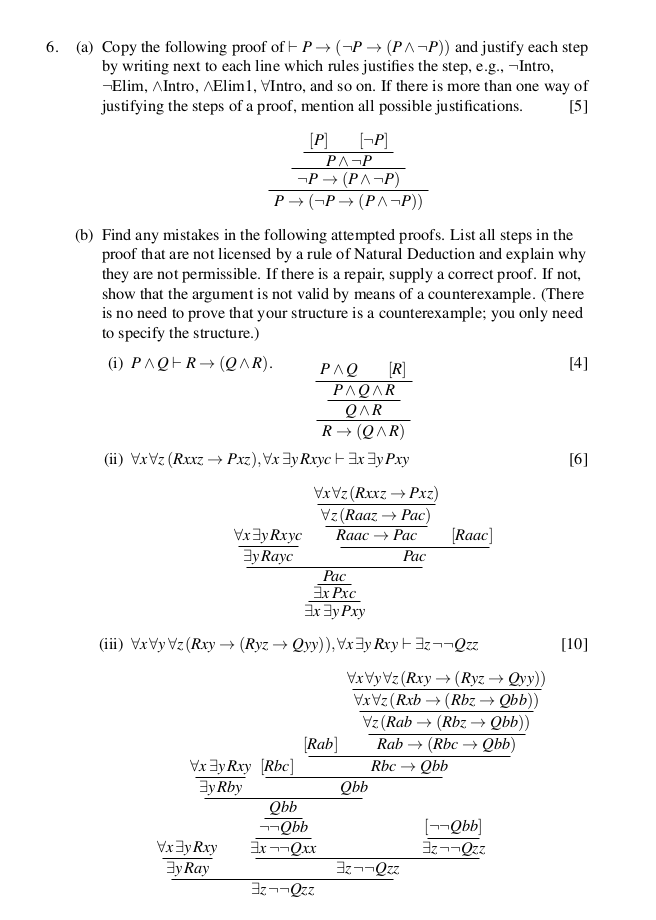
\includegraphics[width=1\textwidth]{Q6.png}
\end{center}

\section*{Solutions}


\vspace{.1in}
\begin{customthm}{(6.b.iii)}
  $ \forall x
      \forall y
        \forall z
          ( Rxy \rightarrow
              ( Ryz \rightarrow Qyy )),
    \forall x
      \exists y Rxy
    \vdash
      \exists z
        \neg\neg Qzz$
\end{customthm}

\begin{Answer}
  \begin{center}
    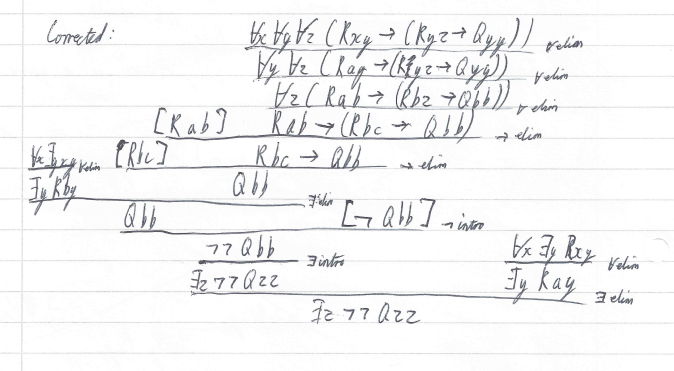
\includegraphics[width=1\textwidth]{6biii.png}
  \end{center}
\end{Answer}






% \vfill

% \bibliographystyle{Phil_Review} %%bib style found in bst folder, in bibtex folder, in texmf folder.
% \bibliography{Zotero} %%bib database found in bib folder, in bibtex folder


\end{document}
